\subsection{Greedy Heuristic Path}\label{sec:greedy}
As mentioned in Section \ref{sec:optiprob} finding an optimal solution to a path is an NP-complete problem. In this section a greedy heuristic approach is proposed which solves the problem one edge at a time. The problem then becomes finding the optimal speed for the current edge, in the interval of $v_{min}$ and $v_{max}$.

Given a path there are two possible cases when choosing the optimal speed for passing an edge:
\begin{enumerate}
	\item Case 1: Driving is fastest
	\item Case 2: Charging and driving is fastest
\end{enumerate}
The intuition is then to find which speed we want to drive and whether or not we should charge before driving. However, it might not be possible to drive at all, given the limited battery of the EV. 

For case 1: The optimal speed when passing the edge $e_i$ = $(u_i, u_{i+1})$ without charging, can be found by solving this equation for $v$:
\[B_{cur} - D(e_i) \times R_{CO}(v) = 0\] 
We call this speed $v_{opt1}$. If $v_{opt1}$ is lower than $v_{min}(e_i)$, there is not enough energy in the battery to drive from $u_i$ to $u_{i+1}$ and thus the time is set to $\infty$, indicating that just driving is not an option. If it is possible to drive the edge using only energy from the battery, the time it will take to pass the edge can be calculated as $D(e_i) / v_{opt1}$

For case 2: The equation for solving an edge, $e_i$, when driving and charging is given by the following equation: 
\begin{equation*}
\begin{aligned}
T(v) = \frac{D(e_i)}{v} + \frac{R_{CO}(v) \times D(e_i) - B_{cur}}{charge_{rate}(u_{i})}
\end{aligned}
\end{equation*}
This equation is on the form: $av^2 + bv + c$, due to the fact that $R_{CO}(v)$ is a quadratic function. $a$, $b$ and $c$ are some constants which are given by the instance of the vehicle. Represented in a Cartesian coordinate system, $T(v)$ is a parabola, as can be seen in Figure \ref{fig:graph}, note that the graph is only defined for positive speeds larger than $0$ and can only be calculated if $charge_{rate}(u_{i})$ is larger than $0$. On the x-axis is the speed of the vehicle and on the y-axis is the time spent. The turning point of the graph represents the optimal speed, $v_{opt2}$, to pass $e_i$. The turning point is easily calculated by finding a tangent line with a slope of $0$.  

\begin{figure}[!htb]
\label{fig:graph}
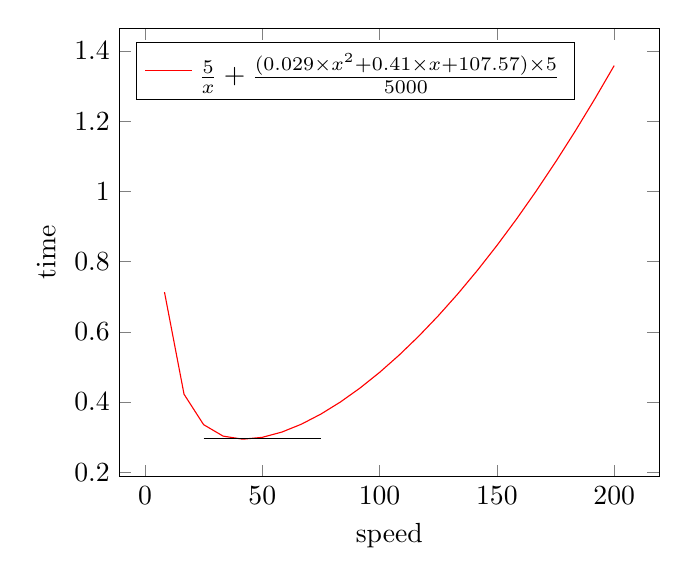
\begin{tikzpicture}
\begin{axis}[xlabel=speed, ylabel=time,legend style={legend pos=north west}]
\addplot[draw=red,domain=0:200]{(5/x)+(((0.0286*x^2 + 0.4096*x + 107.57)*5)/5000)};
\addlegendentry{$\frac{5}{x}+\frac{(0.029\times x^2 + 0.41\times x + 107.57)\times 5}{5000}$}

\addplot[draw=black,domain=25:75]{0.295};
% \addplot[mark=*, domain=25:75] coordinates {(37,295)};
\end{axis}
\end{tikzpicture}% 
\caption{In this instance of $T(v)$, going from $u_i$ to $u_{i+1}$, we have a distance of $5 \si{\km}$ and a charge speed of $5 \si{\kW}$ on $u_i$. The optimal speed in this case is $42.12\si{\km\per\hour}$, and the total time is roughly 17 minutes to pass through the edge when driving and charging}
\label{fig:graph}
\end{figure}

If $v_{opt2}$ is smaller than $v_{min}(e_i)$, then $v_{min}(e_i)$ defines the optimal speed for the edge. Similarly if $v_{opt2}$ is larger than $v_{max}(e_i)$, $v_{max}(e_i)$ defines the optimal speed for the edge. If $v_{opt2} = v_{min}(e_i)$ there might be a possibility that driving and charging is not an option. The time when passing edge $e_i$ in case 2, can then be found with $T(v_{opt2})$.

Having the two ways of deciding the time it takes to pass an edge, we can formulate an algorithm which decides how to drive each edge:

\begin{algorithm}[!htb]
 \begin{algorithmic}[1]
  \Function{travel\_time}{$RN, u_1, u_2, EV$}
    \State $f_{drive} = EV.B_{cur}-RN.D(e)\times EV.R_{CO}(v)$
    \State $f_{charge-drive} = RN.D(e)/v + (RN.D(e)\; \times$
    \XState{$EV.R_{CO}(v)-energy)/charge\_rate)$}
  	\State $e = (u_1, u_2)$
  	\State $v_{opt1} = solve1(v, f_{drive})$
  	\If{$ EV.B_{cur} - RN.D(e)\times EV.R_{CO}(v_{opt1}) < 0 $}
  		\State $time_1 = \infty$
  	\Else
 		\State $time_1 = RN.D(e) / v_{opt1}$
 		\State $energy\_needed_{1} = RN.D(e)\times EV.R_{CO}(v_{opt1})$
  	\EndIf
		\State $CS = getCS(u_1)$ 
  		\State $energy\_needed_{2} = \infty$
  		\State $energy = EV.B_{cur}$
  		\State $time\_added = 0$
  		\State $time_2 = \infty$
  	\While{$energy\_needed_{2} > energy  \And  len(CS) \neq 0$}
  		\State $best_{CS} = extractmax(CS)$
  		\State $B_{possible} = best_{CS}.B_{possible}$
  		\State $charge\_rate = RN.R_{CH}(best_{CS})$
  		\State $v_{opt2} = solve2 (v, f_{charge-drive})$ 
  		\State $energy\_needed_{2} = RN.D(e)\times EV.R_{CO}(v_{opt2})$
  		\State $energy = energy + B_{possible}$
  		\If{$energy - energy\_needed_{2}) < 0$}
  			\State $time\_added = time\_added\; +$
         \XState{$(B_{possible} / charge\_rate)$}
  			\State $CS.remove(0)$
  			\State $updateCS(CS)$
  		\EndIf	
  	\EndWhile
  	\If{$(energy - energy\_needed_{2}) < 0$}
  		\State $time_2 = (RN.D(e)/v_{opt2})\; +$ 
      \XState{$(energy\_needed_{2}/charge\_rate) + time\_added$}
  	\EndIf
  	\If{$time_1 = \infty \And time_2 = \infty$}
  		\State \Return $\infty, \textsc{nil}, \infty, \infty$
  	\EndIf
  	\If{$time_1 \leq time_2$}
  		\State \Return $(time_1, CS,$ 
  		\XState{$EV.B_{cur}-energy\_needed_1, energy\_needed_1)$}
  	\Else
  		\State \Return $(time_2, CS,$ 
  		\XState{$energy - energy\_needed_{2}, energy\_needed_2)$}
  	\EndIf
  \EndFunction
  \end{algorithmic}\caption{The travel time algorithm}\label{alg:travel_time}
\end{algorithm}

The $travel\_time$ function takes as input a road network $RN$, the two vertices which makes up the edge to be driven and an EV. The procedure utilises a few helping functions. The two solve functions $solve1$ and $solve2$ are function solvers specified for case 1 and case 2. The solvers returns the optimal speed for the EV according to the edges driven. 

The function $getCS(u_1)$ returns a list of charging stations. If $u_1$ is a charging stations with a higher charge rate than any charging station previous to $u_1$ in the path, then $u_1$ is returned. Otherwise, the list of charging stations prior to $u_1$ is returned, with the best charging station in the beginning of the list. The function also maintain the potential energy remaining on each charging station. This means that every time the EV spend energy driving, this energy is removed from the potential energy on all charging station. When a charging station is reached, the potential energy is set, based on the difference between the battery capacity and the current battery: $EV.B_{cap}-EV.B_{cur}$. For instance, if the EV reaches a charging station with 50\% battery, the remaining 50\% battery capacity is the potential energy set for that charging station.

The last function $updateCS(CS)$ finds a new best charging station and deletes all charging stations prior to it, this is needed because  previously best charging station has been removed by $CS.remove(0)$. Lines 5-10 handles case 1: Driving using the battery already in the battery. Lines 11-26 handles case 2: Charging and driving. The while loop ranging from line 16 till 26 makes sure the EV always charge as much as possible, at the best previous charging station, but without allowing overcharging. The if statement on line 6 and 27 checks if a valid solution to the case is found, if so, the time for the case is calculated. Lines 29-34 checks if a solution is found and if so, which solution is better. Having a way to solve a single edge, the time of the path can be computed by looping over all edges.



